\documentclass{article}
\usepackage{handover}
\usepackage{placeins}
\usepackage{cleveref}
\usepackage{float}
\usepackage{pgf-umlsd}

\begin{document}
\doctitle{Architecture}{Music Podcast Player}
\FloatBarrier

\section{Core Architecture}
The Music Podcast Player uses a layered service architecture:
\begin{itemize}
\item \textbf{Frontend}: Vue single-page application with routes for user interaction.
\item \textbf{API Service}: Flask REST API for public-facing logic.
\item \textbf{DB Service}: FastAPI internal service for user/playlist persistence logic.
\item \textbf{Data Stores}: PostgreSQL (relational app data), DynamoDB (rate-limiting), S3-compatible object storage (editable page content).
\end{itemize}

\section{Architecture Diagram}

\begin{figure}[H]
\centering
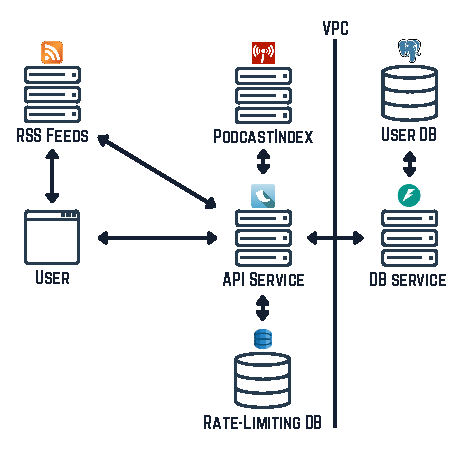
\includegraphics[]{architecture_diagram.pdf}
\caption{Software architecture: frontend, API layer, internal DB service, and data stores.}
\label{fig:arch_diagram}
\end{figure}

\section{Component Responsibilities}
\subsection{Frontend (Vue)}
\begin{itemize}
\item Renders UI and manages user interaction.
\item Calls backend endpoints for auth, search, feed parsing, playlists, and page content.
\item Integrates Lightning wallet actions through Bitcoin Connect.
\end{itemize}

\subsection{API Service (Flask)}
\begin{itemize}
\item Public API boundary and request validation.
\item Exposes route groups: \texttt{/auth}, \texttt{/search}, \texttt{/link}, \texttt{/playlists}, \texttt{/pages}.
\item Applies authorization and rate-limit checks.
\item Orchestrates calls to DB Service and external feed/search providers.
\end{itemize}

\subsection{DB Service (FastAPI)}
\begin{itemize}
\item Encapsulates persistence logic for users and playlists.
\item Handles CRUD operations against relational data models.
\item Returns typed responses to API Service.
\end{itemize}

\subsection{Storage Layer}
\begin{itemize}
\item \textbf{PostgreSQL}: user accounts, playlists, playlist tracks.
\item \textbf{DynamoDB}: token-bucket rate-limit counters and expiry state.
\item \textbf{S3-compatible CMS storage}: editable HTML page payloads by page key.
\end{itemize}

\section{Primary Data Flows}
\subsection{Authentication Flow}
\begin{enumerate}
\item Frontend starts login flow and submits credentials.
\item API Service validates credentials via DB Service.
\item API Service issues access/refresh tokens and uses cookie-based session flow.
\item Frontend verifies/refreshes auth state through auth endpoints.
\end{enumerate}

\subsection{Feed Search and Parsing Flow}
\begin{enumerate}
\item Frontend sends search or feed URL request to API Service.
\item API Service validates request and applies rate-limit logic.
\item API Service calls external integrations for search/parsing.
\item Normalized feed data returns to frontend.
\end{enumerate}

\subsection{Playlist Flow}
\begin{enumerate}
\item Authenticated user performs playlist action from frontend.
\item API Service authorizes and forwards persistence operation to DB Service.
\item DB Service updates PostgreSQL and returns result.
\item API Service may enrich track metadata before returning to frontend.
\end{enumerate}

\subsection{Editable Page Content Flow}
\begin{enumerate}
\item Public reads retrieve page content through \texttt{GET /pages/\{page\}}.
\item Admin edits submit sanitized HTML through \texttt{PUT /pages/\{page\}}.
\item API Service stores/retrieves page JSON in CMS object storage.
\end{enumerate}

\section{Key Design Decisions}
\begin{itemize}
\item \textbf{Service separation}: public API logic is separated from persistence logic for maintainability and clearer boundaries.
\item \textbf{Split backend boundary}: the backend is divided into an API Service and a DB Service. The DB Service is responsible for database access, while the API Service handles public requests and external integrations.
\item \textbf{VPC isolation for database access}: database-connected components are placed inside the VPC so relational data access remains isolated from the public-facing application layer.
\item \textbf{External API access outside the VPC}: the API Service is kept outside the VPC so it can communicate with external services such as the PodcastIndex API without requiring additional VPC egress infrastructure. It then communicates with the DB Service for persistence-related operations.
\item \textbf{Hybrid storage}: relational store for core entities, key-value store for high-churn rate-limit state, object storage for editable static content.
\item \textbf{Backend-mediated integrations}: external feed/search interactions are centralized in backend services for consistent validation and error handling.
\item \textbf{Cookie-based auth}: simplifies frontend token handling and supports secure, session-like UX.
\end{itemize}

\section{Authentication Architecture}
The application uses cookie-based authentication with a PKCE-protected login flow. When the login page loads, the frontend generates a PKCE verifier/challenge pair. The verifier is stored in browser session storage, while the challenge is sent to the backend and stored in the server-side session. During login, the frontend submits the username, password, and verifier. The backend validates the credentials, recomputes the challenge from the verifier, and confirms that it matches the stored challenge before issuing authentication cookies.

\begin{figure}[H]
\centering
\small
\begin{sequencediagram}
  \newinst{u}{User}
  \newinst{f}{Frontend}
  \newinst{a}{API Service}
  \newinst{d}{DB Service}

  \begin{call}{u}{1 Open login}{f}{}
  \end{call}

  \begin{call}{f}{2 Send challenge}{a}{}
  \end{call}

  \begin{call}{u}{3 Submit creds}{f}{}
  \end{call}

  \begin{call}{f}{4 POST /auth/login + verifier}{a}{}
    \begin{call}{a}{5 Check creds}{d}{6 Result}
    \end{call}
    \begin{callself}{a}{7 Verify PKCE}{}
    \end{callself}
  \end{call}

  \begin{call}{a}{8 Cookies or error}{f}{}
  \end{call}
\end{sequencediagram}

\vspace{0.4em}
\footnotesize
\begin{tabular}{ll}
1 & User opens login page \\
2 & Frontend sends PKCE challenge to backend session \\
3 & User enters username and password \\
4 & Frontend sends credentials and PKCE verifier \\
5-6 & API validates credentials through DB service \\
7 & API verifies verifier against stored challenge \\
8 & API sets auth cookies on success, else returns error \\
\end{tabular}

\caption{PKCE login flow}
\label{fig:pkce_sequence}
\end{figure}

This design binds the login request to the browser session that initialized authentication and separates credential validation from token issuance.

\end{document}